\section{Content}
\label{section:content}

\subsection{DDoS Attacks and BRO}\label{subsec:ddos-and-bro}
In this section we will first define the notion of a DDoS attack by explaining how the infrastructure looks like. Then we will elaborate on various DDoS attacks used nowadays and discuss their main characteristics. After this we will discuss the syntax of the detection rules of the BRO SIDS.

\subsubsection{The DDoS Attack}
Figure \ref{fig:ddos-overview} shows the infrastructure of a DDoS attack. Actors involved in a DDoS attack are denoted by a letter (A-D) whereas data streams are denoted by numbers (1-5). 

A DDoS attack starts with an attacker (A). The attacker sends data needed to start the attack (1) to the Command and Control (C\&C) servers (B). The C\&C servers control the infected machines (C). The infected machines are also known under the name of bots. The C\&C servers plus the infected machines are more commonly named as a botnet. The C\&C servers send a message (2) to the infected machines. In case of the Ramnit botnet, only the infected machines counted 3.2 million machines \cite{europol2015}. At this point two paths are used to get to the target machine (E). The first path possible is aiming the infected machines directly to the target (4). The second path possible is using public services (D) like a DNS to reach the target (5). 

In the next subsection we will describe various types of DDoS attacks. 

\begin{figure}[H]
\centering
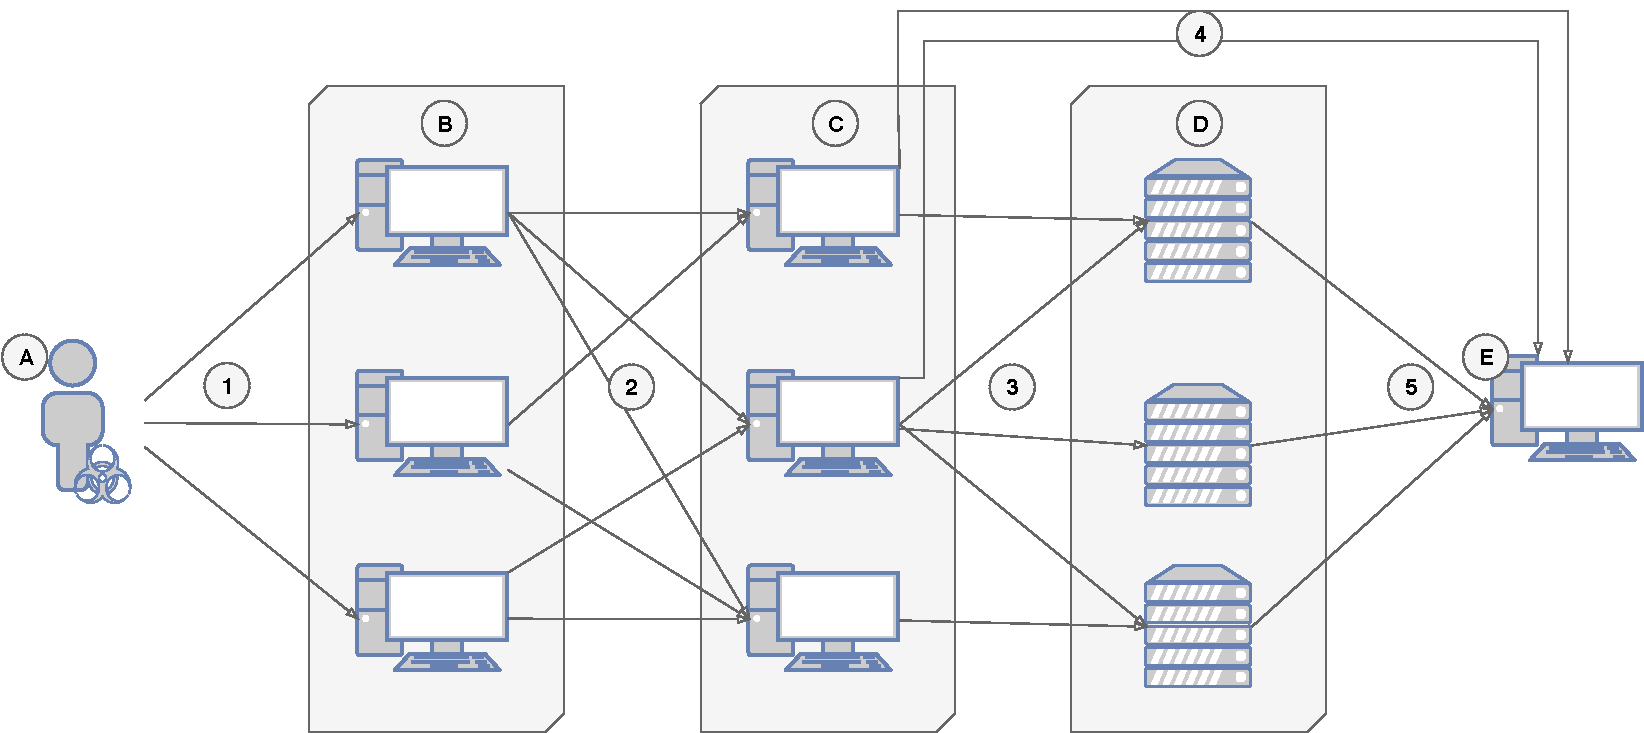
\includegraphics[width=\textwidth]{./images/ddos-overview.pdf}
\caption{Overview of DDoS attack infrastructure}
\end{figure}\label{fig:ddos-overview}

\subsubsection{Types of Attacks}
In this section we will briefly elaborate on the most common types of attack mentioned in the security report of Akami Q4 2017 \cite{Akamai2017-4}. An overview of the main characteristics per attack can be found in Table \ref{tab:attack-overview}.


\paragraph{UDP}
The UDP attack exploits UDP. The attack consists of sending a large number of packets to random ports of the target. Hereby the target machine will check if an application listens to this port and if not will reply with an ICMP Destination Unreachable packet. Looking at Figure \ref{fig:ddos-overview}, path 4 is used.

\paragraph{UDP Fragment}
The UDP Fragmantation attack exploits the fragmentation used in the IP protocol \cite{imperva}. When a packet is to big to be sent across a network link, it will be broken down into smaller packets and later on resembled again. In a UDP Fragmentation attack, fraudulent UDP packets are sent which are larger than the maximum transmission unit (MTU) of the network. The idea is that the packets can not be reassembled and thereby consuming the server's resources. 

\paragraph{DNS}
The DNS attack exploits the public Domain Name System (DNS) services on the internet. DNS is used to resolve IP adresses from website names. In a DNS attack the attacker spoofs its IP replacing its IP with that of the target. The DNS server sees the request as it came from the target and replies as if it were a normal request. This way of attacking allows an attacker to amplify its own bandwidth by using the asymmetry between request and response size. Looking at Figure \ref{fig:ddos-overview}, path 5 is used. The attack runs over UDP.  

\paragraph{NTP}
The NTP attack exploits the public Network Time Protocol (NTP) services on the internet. NTP services allow for time synchronization between machines. This attack is similar to the DNS attack, but this time the NTP services instead of the DNS services are used. 

\paragraph{Chargen}
The Chargen attack exploits the public Character Generator Protocol (Chargen). Once a Chargen services receives a packet via UDP, it responds by sending a datagram containing a random number between 0 and 512 characters long \cite{ietf1983}. The attack approach works the same as the NTP and DNS attacks.  

\paragraph{CLDAP}
The CLDAP attack exploits the Connection-less Lightweight Directory Access Protocol (CLDAP). CLDAP is designed to provide access to directories while not needing the recourse requirements of the Directory Access Protocol (DAP) \cite{ietf1995}. The attack is similar to the DNS, NTP and Chargen attack. 

\paragraph{SYN}
The SYN attack exploits the three-way handshake of TCP. During this attack a large number of SYN packets are send to the target machine. The target machine will respond by sending a SYN-ACK packet. The attacker at this point does not respond by sending an ACK packet, leaving the connection half initialized. This way the attacker keeps connections from being used by legitimate users. Compared to the attacks mentioned above, this one runs over TCP rather than UDP. In this attack, path 4 is used. 

\paragraph{SSDP}
The SSDP attack exploits the Simple Service Discovery Protocol (SSDP). SSDP is used to discover network services. The attack is similiar to DNS, NTP and Chargen but when looking to Figure \ref{fig:ddos-overview} the machines in D are for instance home routers, printers or other IOT devices rather than a dedicated server. 


\paragraph{ACK}
The ACK attack exploits TCP. During this attack a large number of ACK packets are send towards the target. These ACKs do not belong to any connection and are therefore dropped at the target machine. This however does deplete resources of the target. The attack runs via path 4.  


\paragraph{RPC}
?

\paragraph{HTTP}
Rather than the attacks mentions above, the HTTP attack targets the application layer. The attack consists of sending a large number of HTTP requests (like GET, PUSH and POST) to the target, hereby depleting its resources. Looking at Figure \ref{fig:ddos-overview}, path 4 is used.



\begin{table}
\centering
\begin{tabular}{l | l}
Attack Type & Main Characteristics \\ \hline \hline
UDP Frag & IPv4 \&\& fragments \\ \hline
DNS & UDP \&\& src\_port==53 \&\& DNS\_query \&\& DNS\_type \\ \hline
CLDAP & UDP \&\& src\_port==389 \\ \hline
NTP & UDP \&\& src\_port==123 \\ \hline
UDP & UDP \\ \hline
Chargen & UDP \&\& src\_port==19 \\ \hline
SYN & TCP \&\& flag==SYN \\ \hline
SSDP & UDP \&\& src\_port==1900 \\ \hline
ACK & TCP \&\& flag==ACK \\ \hline
RPC & ? \\ \hline
HTTP & HTTP \&\& HTTP\_request \&\& src\_port==80
\end{tabular}
\caption{\label{tab:attack-overview}Attack types main characteristic overview.}
\end{table}


\subsubsection{Bro Rule Syntax} 
This section discusses the parts used of the Bro signature framework \footnote{\url{https://www.bro.org/sphinx/frameworks/signatures.html}} and Bro scripting language. 

Bro's primary focus is on its scripting language. With this language one can define various analyzing detection policies. Besides the scripting language, Bro offers also a signature language. This language is similar to Snort rules and rely on low level pattern matching. In this paper we will focus mainly on the Bro signature language to detect various types of DDoS attacks. 

\paragraph{Bro Signature Framework}
The format of a signature is defined in Listing \ref{lst:signature-format}. As can be observed, each signature starts with the \emph{signature} keyword followed by a signature identifier. In the body the attributes to match on and the event that needs to be raised are defined. The used attributes will be explained in the next paragraph. The \emph{event} keyword is used to define a message that is to be passed to the event listener.

\begin{lstlisting}[caption={Bro Signature Format}, label={lst:signature-format}]
signature [SIGNATURE-ID] {
  ATTRIBUTES  
  event "message to display"
}
\end{lstlisting}


\paragraph{Bro Attribute Rules}
An attribute rule has format defined in Listing \ref{lst:attribute-format}. Here \emph{KEYWORD} indicates a certain field to match, \emph{CMP} indicates the way to compare and \emph{VALUE} indicates the value to compare to. Each element of the attribute rule is explained below.

\begin{lstlisting}[caption={Bro Signature attribute rule format}, label={lst:attribute-format}]
KEYWORD CMP VALUE
\end{lstlisting}

Various keywords are known to the Bro signature language. We will briefly discuss the ones used in this research. \emph{src-ip} and \emph{dst-ip} specify the source and destination address respectively. Addresses can be IPv4 or IPv6. \emph{src-port} and \emph{dst-port} specify the source and destination port respectively. \emph{ip-proto} specifies the protocol used. Values possible are: \emph{tcp, udp, icmp, icmp6, ip} and \emph{ip6}. It is also possible to define a general condition to match on the header of the packet. This allows to compare on specific parts of the header. An example of how the keyword can look is given in Listing \ref{lst:header-condition}. First the attribute rule starts with the keyword \emph{header}. Then the protocol is specified (which can be any of the ip-proto values mentioned earlier). Then one defines within the square brackets the offset and size in bytes separated by a colon. In the example an offset of 0 and size of 1 is defined which indicates in the ICMP protocol the type. 

\begin{lstlisting}[caption={Bro Signature header condition}, label={lst:header-condition}]
header icmp[0:1]
\end{lstlisting} 

Bro Signature Framework has various comparator to match packets on. For instance, it is possible to specify that a certain address needs to be higher than a certain value. In our research, we only used the \emph{==} comparator.

   



\paragraph{Bro Scripting Language}
One can define an email address to which a message is sent whenever a signature is matched. This, however, is not suitable for our intended research. Therefore we also need to define our own Bro script in order to receive an adequate message that a signature is matched. The script used can be found in Listing $\dots$. This script is responsible for loading the signatures as well as executing a python script whenever a packet is matched against a signature. The contents of the python script will be explained in Section \ref{subsec:methodology}. 

The Bro script has some things to note. The first is the \emph{@load-sigs ./sig} line. This line is responsible for loading the signatures files. The second is the \emph{event signature\_match($\dots$)} line. This rule illustrates the event-driven programming script of Bro. Whenever a signature is matched, the contents defined within the curly brackets is executed. The \emph{msg} parameter is given the value specified by the event keyword in the signature.  




\subsection{Methodology}\label{subsec:methodology}
In this section we will discuss the test setup used to achieve the results presented and discussed in Section \ref{subsec:evaluation-discussion}.

For this research we created a test setup which is schematically shown in Figure \ref{fig:test-setup}. This setup knows 4 actors. The first actor (1) is the attacker. The second actor (2) is a router. The attacker is directly connected via cable to this router to not hinder any other networks. The third actor (3) is a switch that allows port mirroring. The fourth actor (4) is the target machine. The fifth and final actor (5) is the Bro machine: the machine that runs the Bro IDS. The Bro machine receives all egress packets of the target machine. 


\begin{figure}[H]
\centering
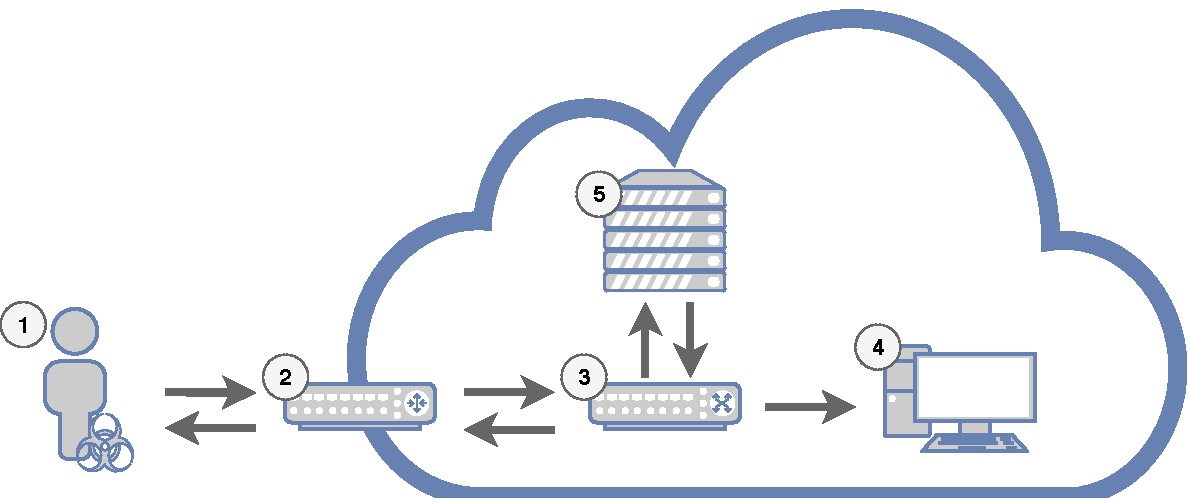
\includegraphics[width=\textwidth]{./images/test-setup.pdf}
\caption{Schematic overview test setup}
\end{figure}\label{fig:test-setup}

For this research we choose 8 attacks to test against our setup. Each attack has a pcap file which contains only the data captured from an actual attack. From this, DDoSDB generated a json file which describes the main attack vectors used in that attack. Each attack has been assigned a four digit identifier to which we will refer to further on in this paper. A brief summary of each attack based on the received json file can be found in Table \ref{tab:json-summarry}.  


\begin{table}[H]
\centering
\begin{tabular}{l | l | l | l | l | l}
ID & Type & \# src IPs & \# src ports & \# dst ports & special  \\ \hline \hline
e0b2 & ICMP & 83 & 0 & 0 & icmp\_type = 5 \\ \hline
0292 & TCP & 6 & 1 & 1 & tcp\_flags = ··········S· \\ \hline
dd26 & Chargen & 439 & 1 & 5 &  \\ \hline
e6ee & DNS & 25027 & 1 & 60219 & dns\_query = hoffmeister.be \\ \hline
54a7 & ICMP & 270 & 2821 & 1 & icmp\_type = 11 \\ \hline
8219 & UDP & 12 & 1 & 96 &  \\ \hline
39b6 & TCP & 66610 & 41757 & 1 & tcp\_flags = ············ \\ \hline
13c4 & UDP & 12 & 1 & 83 &  \\ \hline
c606 & TCP & 13452 & 12110 & 1 & tcp\_flags = ····CE····S· \\ \hline
7bf0 & NTP & 1288 & 1 & 11 &  \\ \hline
151e & ICMP & 244 & 12 & 1 & icmp\_type = 3 \\ \hline
9d61 & ICMP & 6245 & 0 & 0 & icmp\_type = 3 \\ \hline
072a & DNS & 30551 & 1 & 62591 & dns\_query = diasp.org
\end{tabular}
\caption{\label{tab:json-summarry}Attack charasterics}
\end{table}

To answer the second RQ a python script has been created that generates the signatures for the Bro IDS. This script receives as input a json file received from DDoSDB and converts it to a valid Bro signature rule. Each attack has its own generated signature rule. For each attack the signature is generated on the Bro machine and is measured how long it takes. The results of this can be found in Figure $\dots$.

To answer the third RQ first the maximum bandwidth of the target and Bro machine are determined. This is done using iperf3\footnote{\url{https://iperf.fr/}}. The attacker runs the script: \emph{iperf3 -s} and the other machine runs \emph{iperf3 -c [attacker\_ip] -R}. This way the server sends the data to the connecting machine. Second, the attacker will rewrite the destination ip and mac address of the supplied pcap using tcprewrite\footnote{\url{http://tcpreplay.synfin.net/}}. The command used is \emph{tcprewrite --dstipmap=0.0.0.0/0:[target\_ip]/32 --enet-dmac=[target\_mac] --infile=[supplied\_pcap] --outfile=attack.pcap}. Third, Bro is started in bare mode with the Bro script described in Listing \ref{lst:bro-script}. This way only the needed files are loaded. The command used to start Bro is: \emph{sudo [path\_Bro]/bro -b -i [network\_device] [path\_script]}. Fourth, the attack against the target machine is launched using tcpreplay. The command used to launch the attack is: \emph{sudo tcpreplay -i [network\_device] --mbps=[speed\_limit] attack.pcap}. Fifth and lastly, when a signature match is received, the Bro machine will sent a message to the attacker. The times it took of each attack between launching it and receiving the message are displayed in Figure \ref{fig:response-times}.






\subsection{Evaluation and Discussion}\label{subsec:evaluation-discussion}
In this section we will evaluate and discuss our findings we found by executing the methodology described in Section \ref{subsec:methodology}.

In our first attempt of gathering results we used as the attacker a laptop with Intel i7-4700MQ @ 2.4 GHz with 8 GB of RAM, as router the D-Link DIR-605L, as switch the tp-link TL-SG105E, as target machine a Raspberry Pi 2 and as Bro machine a Raspberry Pi 3 Model B. From iperf we measured a maximum bandwidth of 90 Mbps. The Pi could not handle a single attack vector signature at this speed. We then decided to scale down and concluded that even at a speed of 1 Mbps the Pi could not handle every attack. Therefore we concluded that a Pi is not suitable to run the Bro IDS.  

\pgfplotstableset{
    create on use/mean/.style={create col/mean},
    create on use/stddev/.style={create col/standard deviation},
    create on use/stderror/.style={create col/standard error}
}


\begin{tikzpicture}
  \begin{axis}[xticklabel style={rotate=90}, symbolic x coords={7bf0, 8219, c606, e6ee, 072a, e0b2, 9d61, 54a7, 151e, 0292, 39b6, 13c4, dd26, 7bf0, 8219, c606, e6ee, 072a, e0b2, 9d61, 54a7, 151e, 0292, 39b6, 13c4},
xtick={7bf0, 8219, c606, e6ee, 072a, e0b2, 9d61, 54a7, 151e, 0292, 39b6, 13c4, dd26, 7bf0, 8219, c606, e6ee, 072a, e0b2, 9d61, 54a7, 151e, 0292, 39b6, 13c4}, xticklabel style={text height=2ex}, xlabel={Attack Identifier}, ylabel={Time in seconds}, title={Response Times Single Signature},title style={xshift=1.5em, yshift=-1.5ex}]
    \addplot+[only marks, 
            error bars/.cd,
        y dir=both,
        y explicit
    ]
    table[
            x=Sample,
            y=mean,
            y error=stderror
    ]
    {results/data-attacker-single-sigs.txt};
  \end{axis}
\end{tikzpicture}

\begin{tikzpicture}
  \begin{axis}[xticklabel style={rotate=90}, symbolic x coords={7bf0, 8219, c606, e6ee, 072a, e0b2, 9d61, 54a7, 151e, 0292, 39b6, 13c4, dd26, 7bf0, 8219, c606, e6ee, 072a, e0b2, 9d61, 54a7, 151e, 0292, 39b6, 13c4},
xtick={7bf0, 8219, c606, e6ee, 072a, e0b2, 9d61, 54a7, 151e, 0292, 39b6, 13c4, dd26, 7bf0, 8219, c606, e6ee, 072a, e0b2, 9d61, 54a7, 151e, 0292, 39b6, 13c4}, xticklabel style={text height=2ex}, xlabel={Attack Identifier}, ylabel={Time in seconds}, title={Response Times All Signature},title style={xshift=1.5em, yshift=-1.5ex}]
    \addplot+[only marks, 
            error bars/.cd,
        y dir=both,
        y explicit
    ]
    table[
            x=Sample,
            y=mean,
            y error=stderror
    ]
    {results/data-attacker-all-sigs.txt};
  \end{axis}
\end{tikzpicture}









